\documentclass[10pt]{article}
\usepackage[margin=1.4in]{geometry}

% Basic
\usepackage[utf8]{inputenc}
% \usepackage[spanish,mexico]{babel}

\usepackage{parskip}
\usepackage{float}
\usepackage[svgnames]{xcolor}
\usepackage{listings}

\lstset{language=R,
    basicstyle=\small\ttfamily,
    stringstyle=\color{DarkGreen},
    otherkeywords={0,1,2,3,4,5,6,7,8,9},
    morekeywords={TRUE,FALSE},
    deletekeywords={data,frame,length,as,character},
    keywordstyle=\color{blue},
    commentstyle=\color{DarkGreen},
}
\lstdefinestyle{myCustomMatlabStyle}{
  language=Matlab,
  numbers=left,
  stepnumber=1,
  numbersep=10pt,
  tabsize=4,
  showspaces=false,
  showstringspaces=false
}

% Custom colors
\usepackage{color}
\definecolor{deepblue}{rgb}{0,0,0.5}
\definecolor{deepred}{rgb}{0.6,0,0}
\definecolor{deepgreen}{rgb}{0,0.5,0}

% Default fixed font does not support bold face
\DeclareFixedFont{\ttb}{T1}{txtt}{bx}{n}{10} % for bold
\DeclareFixedFont{\ttm}{T1}{txtt}{m}{n}{10}  % for normal

% Python style for highlighting
\newcommand\pythonstyle{\lstset{
language=Python,
basicstyle=\ttm,
otherkeywords={self},             % Add keywords here
keywordstyle=\ttb\color{deepgreen},
emph={MyClass,__init__},          % Custom highlighting
emphstyle=\ttb\color{deepred},    % Custom highlighting style
stringstyle=\color{deepgreen},
frame=tb,                         % Any extra options here
showstringspaces=false            %
}}
% Python environment
\lstnewenvironment{python}[1][]
{
\pythonstyle
\lstset{#1}
}{}


\usepackage{booktabs}
\usepackage{hyperref}
\usepackage{csquotes}
\usepackage{enumitem}

% Math stuff
\usepackage{amsmath, amsfonts, mathtools, amsthm, amssymb}
\usepackage{gensymb}
\usepackage{siunitx}



% Headers
\usepackage{fancyhdr}
\usepackage{lastpage}
\pagestyle{fancy}
\setlength{\headheight}{40pt}

% Commands
\newcommand\N{\ensuremath{\mathbb{N}}}
\newcommand\R{\ensuremath{\mathbb{R}}}
\newcommand\Z{\ensuremath{\mathbb{Z}}}
\newcommand\Q{\ensuremath{\mathbb{Q}}}
\newcommand\C{\ensuremath{\mathbb{C}}}

%Images
\usepackage{import}
\usepackage{xifthen}
\usepackage{pdfpages}
\usepackage{transparent}

\newcommand{\incfig}[1]{%
    \def\svgwidth{\columnwidth}
    \scalebox{.75}{\import{./figures/}{#1.pdf_tex}}
}

\title{Descomposición en valores singulares}
\author{Sergio Arnaud Gómez}
\date{30 de octubre del 2017}

\newtheorem{teo}{Teorema}
\newtheorem{lema}{Lemma}

\newenvironment{solution}
  {\renewcommand\qedsymbol{$\blacksquare$}
  \begin{proof}[Proof]}
  {\end{proof}}
\renewcommand\qedsymbol{$\blacksquare$}


\begin{document}

\lhead{Sergio Arnaud}
\rhead{ Statistical learning (MT7038) \\ Final Project }
\cfoot{\thepage \ of \pageref{LastPage}}

\section{Dataset}

For this proyect, the dataset chosen was \href{https://archive.ics.uci.edu/ml/datasets/Combined+Cycle+Power+Plant}{\textit{Combined Cycle Power Plant Data Set}}. According to the datasets information:

\begin{displayquote}
A combined cycle power plant is composed of gas turbines, steam turbines and heat recovery steam generators. In a CCPP, the electricity is generated by gas and steam turbines, which are combined in one cycle, and is transferred from one turbine to another. While the Vacuum is colected from and has effect on the Steam Turbine, he other three of the ambient variables effect the GT performance.
\end{displayquote}

My main motivation to use this dataset was that the last month there was a \href{https://www.kaggle.com/c/ashrae-energy-prediction/overview}{kaggle} challenge (ASHRAE - Great Energy Predictor III) that tried to answer the question: 'How much energy will a building consume?'. I think this kind of problems dealing with the estimation of energy production and consumption will start to appear more and more and I personally find them to be both really interesting and challenging.

Furthermore, I think that the data was complicated enough to challenge common regression techniques yet simple enough to be solved without advanced domain knowledge or the requirement of more advanced modelling habilities.
\section{Features}
The dataset contains 9568 observations collected from a CCPP over the period 2006-2011 and the features consist of:
\begin{center}
    \begin{tabular}{ |p{5.5cm}||p{2.25cm}|p{2.25cm}|p{1.8cm}|}
     \hline
     Feature name & Min & Max & Data type \\
     \hline
     Temperature (AT)              & 1.81 \degree C & 37.11\degree C & Continous \\
     Ambient Pressure (AP)         & 992.89 mb  & 1033.30 mb   & Continous \\
     Relative Humidity (RH)        & 25.56\%   &  100.16\% &  Continous \\
     Exhaust Vacuum (V)            & 25.36 cm Hg  & 81.56 cm Hg &   Continous \\
     Electrical energy output (PE) & 420.26 MW  & 495.76 MW & Continous \\
     \hline
    \end{tabular}
\end{center}
The individual distribution of each feature is shown in the following figure:
\begin{figure}[H]
    \begin{center}
        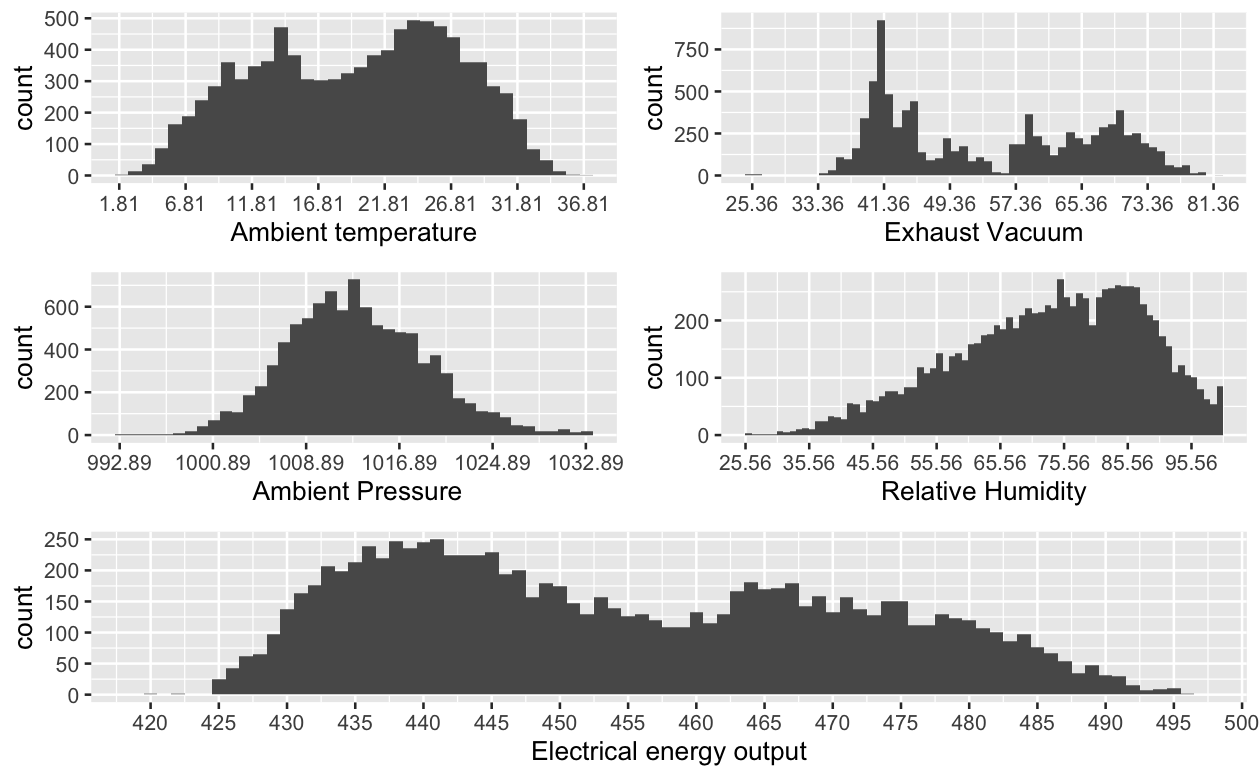
\includegraphics[width=12cm, height=7cm]{img/hist.jpg}
        \caption{Histogram of the variables}
    \end{center}
\end{figure}
\newpage
Both the ambient temperature and the electrical energy output seem to have a bimodal distribution, the relative humidity is unimodal with a negative skew, the ambient pressure appears to be normally distributed and the exhaust vacuum shows the most complicated distribution with several distinct modes.
\section{Relations of the predictors with the response variable}
First, let's take a look to the correlation matrix:
\begin{center}
    \begin{tabular}{ |p{.75cm}|p{.75cm}|p{.75cm}|p{.75cm}|p{.75cm}|p{.75cm}|}
     \hline
      & PE & AP & RH & V & AT \\
     \hline
     PE & 1 &  &  &  & \\
     \hline
     AP & .52 & 1 &  &  & \\
     \hline
     RH & .39 & .1 & 1 &  & \\
     \hline
     V & -.87 & -.41 & -.31 & 1 & \\
     \hline
     AT & -.95 & -.51 & -.54 & .84 & 1\\
     \hline
    \end{tabular}
\end{center}
the response variable has a high negative correlation with both the ambient temperature and the exhaust vacuum, also those features are highly correlated between them.

Now, let's focus on the individual relations of the predictors with the response variable:
\begin{figure}[H]
    \begin{center}
        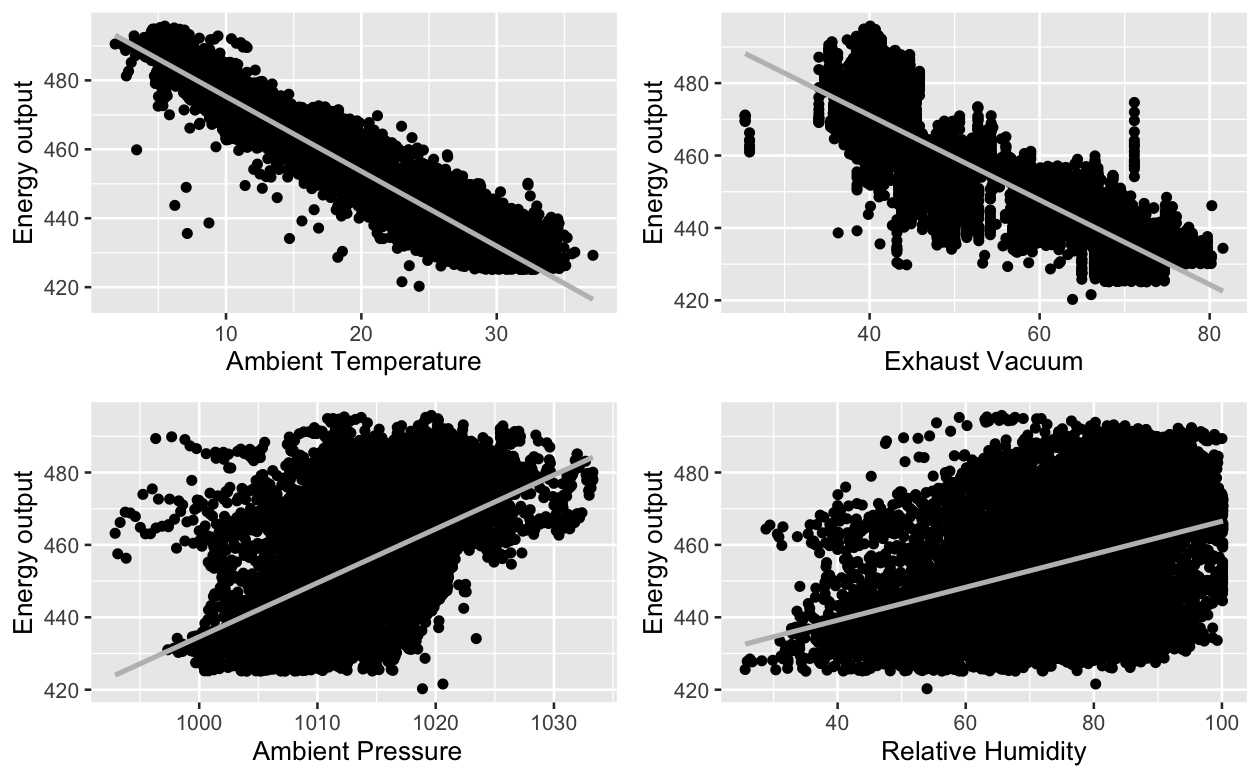
\includegraphics[width=0.8\textwidth]{img/relations.jpg}
        \caption{Individual relations of predictors with response}
    \end{center}
\end{figure}
There's a clear relationship between the temperature and the energy output: for a higher temperature, a lower energy output corresponds. Also the exhaust vacuum appear to show a relationship of that kind. We can't extract any conclusions from the ambient pressure and the relative humidity from this figure.

To finish the analysis of our features, it's important to mention that the data have no misssing values and it looks like we don't have to deal with outliers or further cleaning so we'll just standardize each variable and proceed with the modelling.
\newpage

\section{Modelling}

All the predictors and the response are continuous variables so the task for this dataset is a regression.

A gradient boosted decision tree was used to solve the regression task since I think it's a good fit for the problem in hand and personally wanted to explore and learn more about this particular method.

A more simple and interpretable model was used as a baseline to compare the performance of the gradient boosting model. A linear regresion was fitted, lasso and ridge methods were tried but multicollinearity weren't a problem and the improvement in terms of test error was minimal so I decided in favor of the more simple linear regresion.

\section{Software}
Tha programming language used for the analysis of the CCPP dataset was R and the following table describes the main packages and libraries utilized:
\begin{center}
    \begin{tabular}{ |p{4cm}||p{10.5cm}|}
         \hline
         Library & Description \\
         \hline
         \href{https://www.tidyverse.org}{\textit{Tidyverse}} & For data manipulation and visualization. \\
         \href{http://topepo.github.io/caret/index.html}{\textit{Caret}} (Classification And Regression Training) &  The package goal is to provide a uniform interface to standardize common modelling tasks such parameter tuning and variable importance. In particular, \textit{caret} was used for the cross validation procedure.  \\
         \href{https://xgboost.ai/about}{\textit{XGBoost}}(Extreme Gradient Boosting) & An optimized distributed library which provides a gradient boosting framework for several programming languages including R. \\
         \href{https://www.rdocumentation.org/packages/xgboostExplainer/versions/0.1}{xgboostExplainer} & An R package which allows the predictions from an XGBoost model to be split into the impact of each feature, making the model more interpretable. \\
         \hline
    \end{tabular}
\end{center}

\section{Linear model}
The linear regresion model was straightforward, all the predictors were significant to the response and a significant regression equation was found $(F(4,7651) = \num{2.517e-4}, p < \num{2.2e-16})$ with an $R^2 = 0.9294$.

\section{Gradient boosted decision tree}

Using the library XGBoost a gradient boosted decision tree model was fitted to predict the electrical energy output. The first issue to solve was how to pick the optimal hyperparameters of the model.

\subsection{Parameter tuning}

According to XGBoost there are many hyperparameters to be tuned. The following table resumes the most important, it's meaning, and the value used.

\begin{tabular}{ |p{2cm}||p{11cm}| p{1cm}|}
\hline
Parameter & Description & Value\\
\hline
eta & After each boosting step, eta shrinks the feature weights to make the boosting process more conservative and less likely to overfit & .1 \\
gamma & Minimum loss reduction required to make a further partition on a leaf node of the tree. A larger gamma implies a more conservative algorithm. & 0 \\
max\_depth & Maximum depth of a tree. Increasing this value will make the model more complex and more likely to overfit. & 6 \\
min\_child \_weight & If the tree partition step results in a leaf node with the sum of instance weight less than min\_child\_weight, then the building process will give up further partitioning. & 2\\
\hline
\end{tabular}

To select, eta, max\_depth and min\_child\_weight a grid search was performed and the optimal values were selected with 5 fold cross-validation using caret \textit{train} function. After selecting the optimal hyperparameters, the optimal number of rounds for boosting was found to be 600.

\subsection{Model training and evaluation}
With those parameters, the \textit{xgb.train} function was used to train the optimal model. The test mean squared error was $0.032$ and, as seen in the predicted vs actual energy output plot the predictions are really good.

\begin{figure}[H]
    \begin{center}
        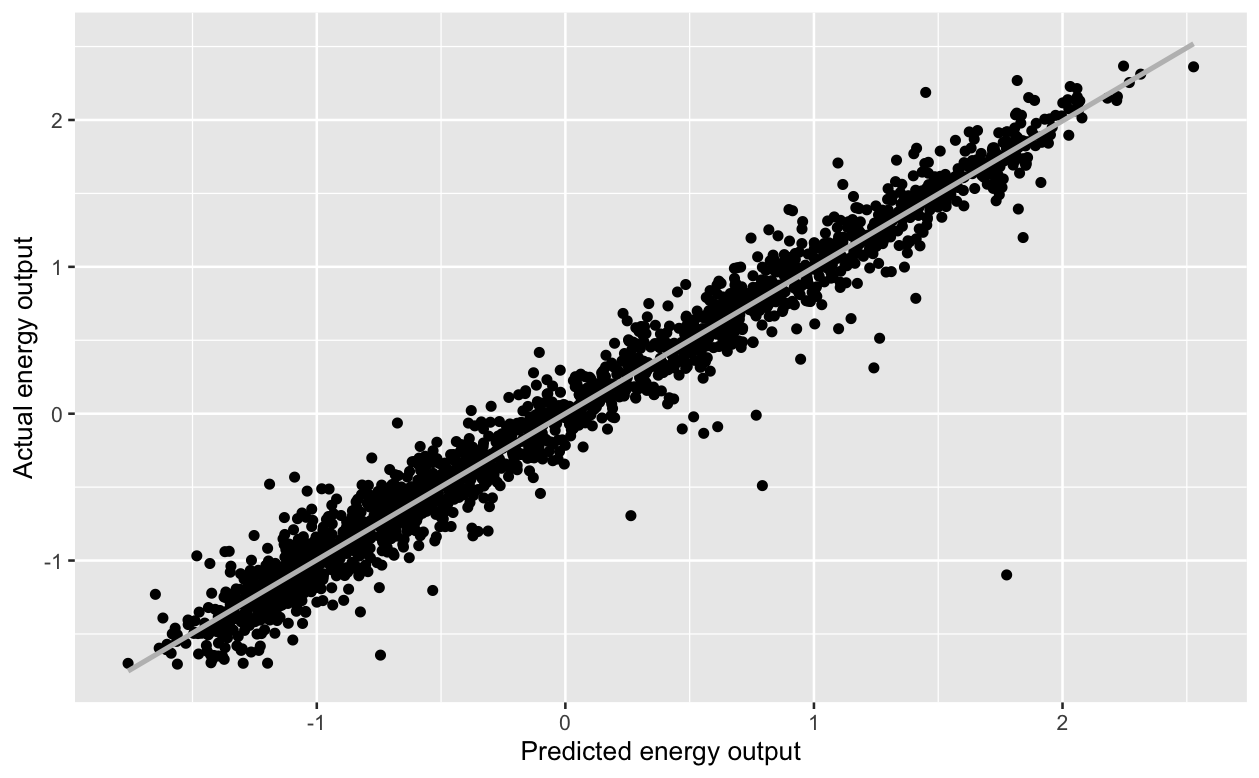
\includegraphics[width=0.8\textwidth]{img/pred_act.jpg}
        \caption{Actual vs Predicted energy output}
    \end{center}
\end{figure}

\subsection{Feature importance}

After the boosted trees are constructed, we can build an importance score for each attribute. That score indicates how valuable each feature was in the fitting process. With the function \textit{xgb.importance}, the following importance values were calculated.
\newpage

\begin{center}
    \begin{tabular}{ |p{4cm}||p{3cm}|}
         \hline
         Library & Description \\
         \hline
         Ambient temperature & .90 \\
         Exhaust Vacuum & .06 \\
         Ambient Preassure & .015 \\
         Relative Humidity & .013 \\
         \hline
    \end{tabular}
\end{center}

The ambient temperature is by far the most important feature, followed by the exhaust vacuum. The ambient preassure and the relative humidity weren't very relevant.

\subsection{Interpretation}

Using the The \textit{xgboostExplainer} R package, we can extract the log-odds contribution of each feature in a prediction by adding up the contributions of each one of them for every tree in the ensemble. With that information, we can measure the impact that each feature had in a particular prediction.

Each plot in the following figure shows the values of a predictor plotted against the impact associated with that value.

\begin{figure}[H]
    \begin{center}
        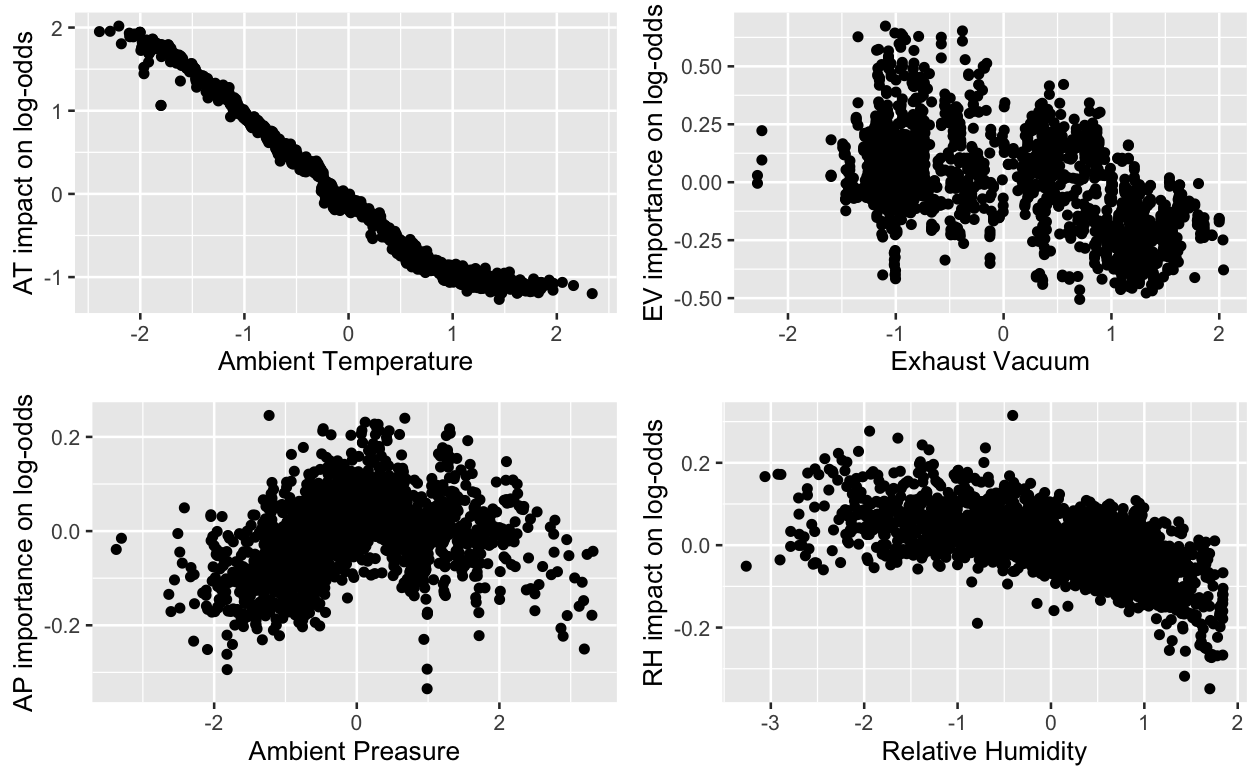
\includegraphics[width=0.9\textwidth]{img/expl_all.jpg}
        \caption{Value vs impact}
    \end{center}
\end{figure}
In the first plot we can see that for lower temperatures the impact is positive (lower temperature contributes to a greater energy output) and as the temperature increases, the impact decreases (a greater temperature contributes to a smaller energy output)

The plot of ambient preassure suggests that, for smaller and bigger values of the preassure the impact to the response is negative (lower and higher preasures lead to an smaller energy output) whilst a mean preassure has, in general, a positive impact (a mean preassure leads to a greater energy output).
\newpage
The plots of exhaust vacuum and relative humidity will be analized with the following graph where each dot is colored with red if the temperature was higher than the mean and blue if it was lower than the
mean.
\begin{figure}[H]
    \begin{center}
        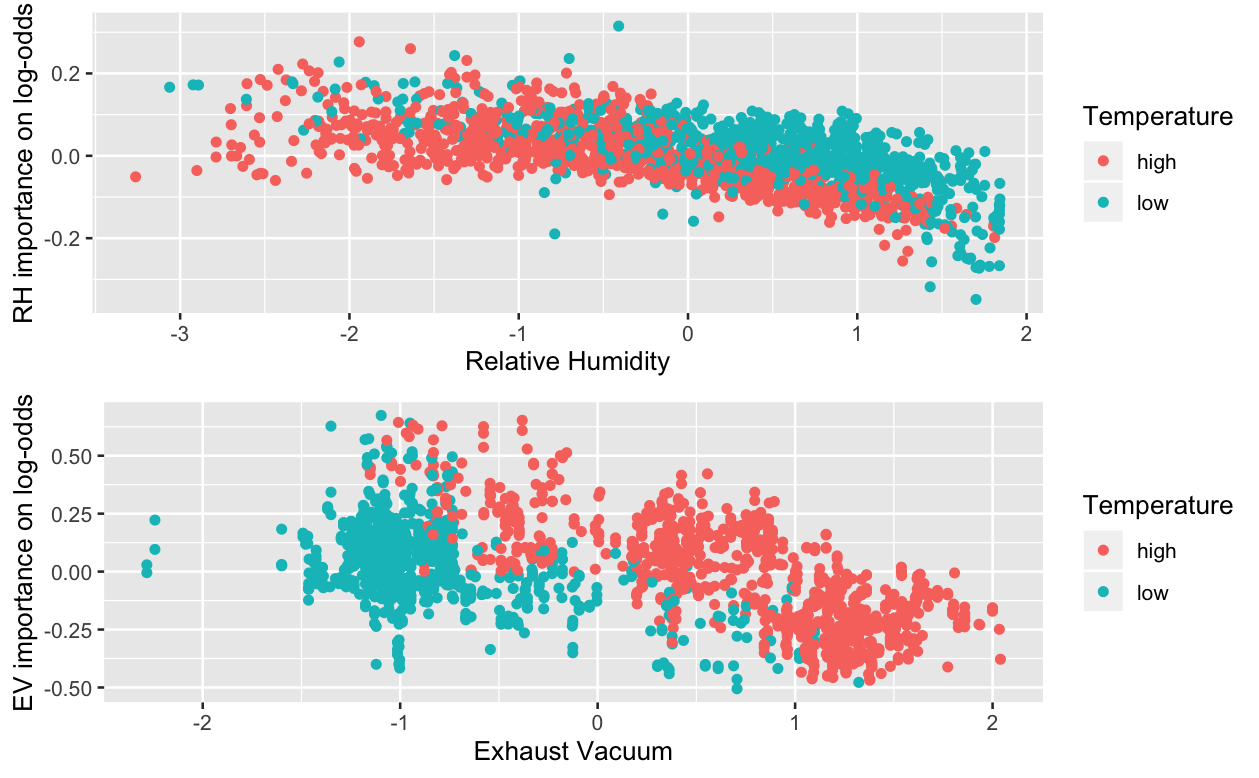
\includegraphics[width=11cm, height=8cm]{img/expl_2}
        \caption{Value vs impact}
    \end{center}
\end{figure}

From the first plot we can see that, for bigger values of humidity we may observe greater energy outputs if the temperature is above the mean; and smaller energy outputs if the temperature is below the mean. A similar analysis can be made for the second plot.

\section{Conclusions}

The linear model achieved good results and is definitely a good alternative to analyze the problem since it's the most interpretable model we could use.

The gradient boosted decision tree model was able to capture some nonlinear relationships between the predictors achieving a mean squared error 76\% smaller than the one from the linear model.

Since the gradient boosting is a complicated model, usually the results lack interpretation. Nevertheless, there exist tools to helps us extract important information about the way in which the model is working and how the predictions are made.

I'm really satisfied with the fact that the gradient boosting model achieves good prediction power without renouncing to interpretation. The gradient boosting framework is, indeed, a very powerfull one.

Posible improvements might involve be in several areas:
\begin{itemize}
    \item The dataset only uses the 4 more common variables in a CCPP, more features could be added for a broader analysis.
    \item The results of both the linear and the gradient boosting models could be further interpreted, maybe with more work and domain knowledge.
    \item Only the main parameters of the gradient boosting model were tuned, we could try doing more exhaustive hyperparameter optimization
    \item Other regression techniques could be tried in order to achieve better predictions or further insights.
\end{itemize}


\end{document}
